\chapter{Details}\label{ch:Details}

\section{Division mit Rest}\label{sec:DivisionMitRest}
\begin{mydefinition}[Kongruenz ganzer Zahlen]
Sei $m > 0$ eine fest gewählte natürliche Zahl. Seien $a$ und $b$ ganze Zahlen. Dann heissen $a$ und $b$ \textbf{kongruent modulo}\index{Kongruenz modulo} $m$, geschrieben
\begin{align*}
	a \equiv b \pmod{m},
\end{align*}
falls $m$ die Differenz $(a - b)$ teilt.
\end{mydefinition}


\begin{mydefinition}[Modulo-Operation]
Sei $m \geq 2$ eine fest gewählte ganze Zahl und $a$ eine ganze Zahl. Dann ist $a$ kongruent modulo $m$ zu genau einer Zahl $b\in\lrc{0, 1, \ldots, m-1}$. Diese Zahl $b$ bezeichnen wir mit dem Ausdruck $a\; \;\%\; \; m$.
\end{mydefinition}

\begin{myexample}\label{myexample:clock}
Auf dem Planeten \textit{Vulcan} dauert ein Tag nur 5 Stunden. Deshalb verwenden die \textit{Vulcanians} Uhren der unten abgebildeten Form. Diese Uhren verfügt lediglich über einen Stundenzeiger.
\begin{figure}[H]
	\centering
	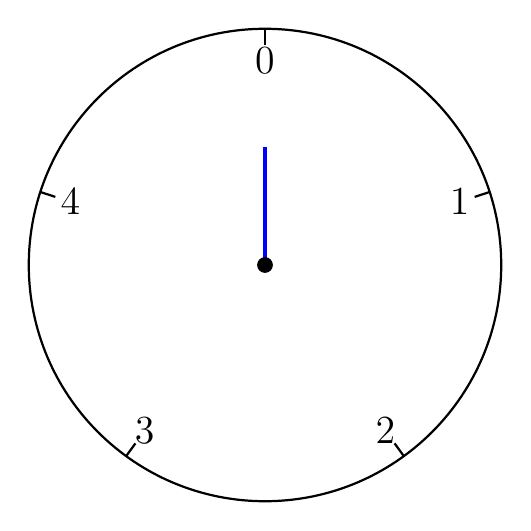
\begin{tikzpicture}
		% Draw the clock circle
		\draw[thick] (0,0) circle (3);

		% Draw the hour marks (5-hour clock)
		\foreach \i in {1,2,3,4,0} {
				\node[font=\Large] at ({90 - \i * 360/5}:2.6) {\i};
				\draw[thick] ({90 - \i * 360/5}:2.8) -- ({90 - \i * 360/5}:3);
			}

		% Draw clock hands
		\draw[very thick, blue] (0,0) -- (0,1.5); % Hour hand

		% Center dot
		\fill (0,0) circle (0.1);
	\end{tikzpicture}
	\caption{Uhr der \textit{Vulcanians}}
\end{figure}

\begin{table}[H]
	\begin{tabular}{|l|l|l|l|l|l|l|l|l|l|l|l|l|l|}
		\hline
		{\color[HTML]{FE0000} vergangene Zeit $T$ in Stunden:} & {\color[HTML]{FE0000} -6} & {\color[HTML]{FE0000} -5} & {\color[HTML]{FE0000} -4} & {\color[HTML]{FE0000} -3} & {\color[HTML]{FE0000} -2} & {\color[HTML]{FE0000} -1} & {\color[HTML]{FE0000} 0} & {\color[HTML]{FE0000} 1} & {\color[HTML]{FE0000} 2} & {\color[HTML]{FE0000} 3} & {\color[HTML]{FE0000} 4} & {\color[HTML]{FE0000} 5} & {\color[HTML]{FE0000} 6} \\ \hline
		{\color[HTML]{3531FF} $T\; \;\%\; \; 5$:}              & {\color[HTML]{3531FF} 4}  & {\color[HTML]{3531FF} 0}  & {\color[HTML]{3531FF} 1}  & {\color[HTML]{3531FF} 2}  & {\color[HTML]{3531FF} 3}  & {\color[HTML]{3531FF} 4}  & {\color[HTML]{3531FF} 0} & {\color[HTML]{3531FF} 1} & {\color[HTML]{3531FF} 2} & {\color[HTML]{3531FF} 3} & {\color[HTML]{3531FF} 4} & {\color[HTML]{3531FF} 0} & {\color[HTML]{3531FF} 1} \\ \hline
	\end{tabular}
	\caption{Es sei die $T$ die ganzzahlige Anzahl der vergangenen Stunden. Dann ist $T\; \;\%\; \; 5$ die Uhrzeit, welche auf der Uhr abgelesen werden kann.}
\end{table}
\end{myexample}

\begin{myexample}[Modulo-Operation]
Wir geben hier einige Beispiele an:
\begin{align*}
	10 \; & \;\%\; \; 7 = 3 \\
	-3 \; & \;\%\; \; 5 = 2 \\
	-17\; & \;\%\; \; 3 = 1 \\
	-7 \; & \;\%\; \; 3 = 2
\end{align*}
\end{myexample}

Falls Sie noch mehr über modulare Arithmetik (und ihre weitreichende Bedeutung) erfahren möchten, empfehlen wir Ihnen wärmstens, das Buch \cite{LearningModernAlgebra} zu studieren.


\section{Umrechnung von Basis \texorpdfstring{$a$}{a} zu Basis \texorpdfstring{$b$}{b} in Python}
Es sei
\begin{align*}
	x = x_nx_{n-1}\ldots x_2x_1x_0 = x_na^n + x_{n-1}a^{n-1} + \ldots + x_2a^2 + x_1a^1 + x_0a^0
\end{align*}
die Darstellung der Zahl $x$ in Basis $a\geq 2$. Wir wollen die Darstellung
\begin{align*}
	x = x'_mx'_{m-1}\ldots x'_2x'_1x'_0 = x'_mb^m + x'_{m-1}b^{m-1} + \ldots + x'_2b^2 + x'_1b^1 + x'_0b^0
\end{align*}
von $x$ in Basis $b\geq 2$ finden. Die  Ziffern $x'_m, \ldots, x'_1, x'_0$ sind gesucht.

Wir berechnen
\begin{align*}
	x\;\%\; b & = (x'_mb^m + x'_{m-1}b^{m-1} + \ldots + x'_2b^2 + x'_1b^1 + x'_0b^0) \;\%\; b =                                              \\
	          & = (x'_mb^m \;\%\; b + x'_{m-1}b^{m-1} \;\%\; b + \ldots + x'_2b^2 \;\%\; b + x'_1b^1 \;\%\; b + x'_0b^0 \;\%\; b) \;\%\; b = \\
	          & = (0 + 0 + \ldots + 0 + x'_0\;\%\;b)\;\%\; b = (x'_0)\;\%\; b = x'_0,
\end{align*}
wobei wir die Formel $(x + y) \;\%\; a = (x\;\%\; a + y\;\%\; a)\;\%\; a$ ohne Beweis verwendet haben. Somit ist $x\;\%\; b = x'_0$ die Ziffer (das Gewicht) des kleinsten Stellenwerts der Zahl $x$ in Basis $b$.

Nun berechnen wir
\begin{align*}
	x^{(1)} & := x // b =  (x'_mb^m + x'_{m-1}b^{m-1} + \ldots + x'_2b^2 + x'_1b^1 + x'_0b^0) // b =     \\
	        & = x'_mb^m // b + x'_{m-1}b^{m-1} // b+ \ldots + x'_2b^2 // b+ x'_1b^1 // b+ x'_0b^0 // b = \\
	        & = x'_mb^{m-1} + x'_{m-1}b^{m-2} + \ldots + x'_2b^1 + x'_1b^0.
\end{align*}
Danach erhalten wir die zweithinterste Ziffer $x'_1$ durch $x^{(1)}\;\%\; b$ und so weiter. In \cref{listing:base_a_to_base_b} ist eine Python-Funktion gegeben, welche die Umrechnung von Basis $a$ in Basis $b$ berechnet.
\clearpage
\lstinputlisting[language=Python,caption=\texttt{base\_a\_to\_base\_b.py},label=listing:base_a_to_base_b]{Grundlagen_Info/00_Programmieren/Skript/Code/K04_Functions/base_a_to_base_b.py}
